\documentclass[a4paper,12pt]{ltxdoc}
\usepackage{lmodern}
\usepackage[T1]{fontenc}
\usepackage[utf8]{inputenc}
\usepackage{hyperref}
\usepackage{parskip}
\usepackage{microtype}
\usepackage{morefloats}
\usepackage[absolute]{textpos}
\usepackage{tabularx}
\usepackage[table]{xcolor}
\usepackage{graphicx}
\usepackage{mathtools}
\usepackage{multirow}
\usepackage{longtable}
\usepackage{sbc-template}
% \usepackage{natbib}
\usepackage{geometry}
  \geometry{
    top=3.5cm,
    left=3cm,
    right=3cm,
    bottom=2.5cm
  }

\usepackage[english,brazil]{babel}
\selectlanguage{brazil}
\addto\captionsbrazil{
  \renewcommand{\bibname}{Refer\^encias}
  \renewcommand{\indexname}{\'Indice}
  \renewcommand{\listfigurename}{Lista de ilustra\c{c}\~{o}es}
  \renewcommand{\listtablename}{Lista de tabelas}
  \renewcommand{\pageautorefname}{p\'agina}
  \renewcommand{\sectionautorefname}{se{\c c}\~ao}
  \renewcommand{\subsectionautorefname}{subse{\c c}\~ao}
  \renewcommand{\paragraphautorefname}{par\'agrafo}
  \renewcommand{\subsubsectionautorefname}{subse{\c c}\~ao}
  \renewcommand{\paragraphautorefname}{subse{\c c}\~ao}
}  

\usepackage{color}
\definecolor{thered}{rgb}{0.65,0.04,0.07}
\definecolor{thegreen}{rgb}{0.06,0.44,0.08}
\definecolor{thegrey}{gray}{0.5}
\definecolor{theshade}{rgb}{1,1,0.97}
\definecolor{theframe}{gray}{0.6}
\definecolor{blue}{RGB}{41,5,195}
\newcommand{\orientador}{Prof. Dr. Pedro Paulo Balbi de Oliveira}
\newcommand\tab[1][1cm]{\hspace*{#1}}
\IfFileExists{listings.sty}{
  \usepackage{listings}
  \lstset{%
    language=[LaTeX]TeX,
    columns=flexible,
    basicstyle=\ttfamily\small,
    backgroundcolor=\color{theshade},
    frame=single,
    tabsize=2,
    rulecolor=\color{theframe},
    title=\lstname,
    escapeinside={\%*}{*)},
    breaklines=true,
    commentstyle=\color{thegrey},
    keywords=[0]{\fichacatalografica,\errata,\folhadeaprovacao,\dedicatoria,\agradecimentos,\epigrafe,\siglas,\simbolos,\citacao,\alineas,\subalineas,\incisos},
    keywordstyle=[0]\color{thered},
    keywords=[1]{},
    keywordstyle=[1]\color{thegreen},
    breakatwhitespace=true,
    alsoother={0123456789_},
    inputencoding=utf8,
    extendedchars=true,
    literate={á}{{\'a}}1 {ã}{{\~a}}1 {é}{{\'e}}1 {è}{{\`{e}}}1 {ê}{{\^{e}}}1 {ë}{{\¨{e}}}1 {É}{{\'{E}}}1 {Ê}{{\^{E}}}1 {û}{{\^{u}}}1 {ú}{{\'{u}}}1 {â}{{\^{a}}}1 {à}{{\`{a}}}1 {á}{{\'{a}}}1 {ã}{{\~{a}}}1 {Á}{{\'{A}}}1 {Â}{{\^{A}}}1 {Ã}{{\~{A}}}1 {ç}{{\c{c}}}1 {Ç}{{\c{C}}}1 {õ}{{\~{o}}}1 {ó}{{\'{o}}}1 {ô}{{\^{o}}}1 {Õ}{{\~{O}}}1 {Ó}{{\'{O}}}1 {Ô}{{\^{O}}}1 {î}{{\^{i}}}1 {Î}{{\^{I}}}1 {í}{{\'{i}}}1 {Í}{{\~{Í}}}1,
  }
  \let\verbatim\relax
  \lstnewenvironment{verbatim}[1][]{\lstset{##1}}{}
}

\titlespacing{\section}      {0pt}{12pt}{10pt}
\titlespacing{\subsection}   {0pt}{12pt}{10pt}
\titlespacing{\subsubsection}{0pt}{12pt}{10pt}

\usepackage{parskip}
\setlength{\parindent}{0pt}
% \parindent 1.27cm
\title{\protect\parbox{\textwidth}{\protect\centering \textbf{\titulo}}}

\date{}

\hypersetup{
  pdftitle={Conservabilidade de estados de autômatos celulares elementares com atualizações assíncronas por prioridade da vizinhança},
  pdfauthor={Marcelo Vironda Rozanti}{Felipe Stefanelli de Aguiar Silva},
  pdfproducer={Marcelo Vironda Rozanti},
  pdfcreator={vim+LaTeX+abnTeX2},
  colorlinks=true,
  linkcolor=black,
  citecolor=black,
  urlcolor=blue
}

\CodelineIndex
\hyphenpenalty=1000

\addto\captionsbrazil{\renewcommand\abstractname{}}
\addto\captionsenglish{\renewcommand\abstractname{}}

\usepackage{courier}
% \renewcommand{\ttdefault}{pcr}
\begin{document}

% \pagestyle{empty}
% \pagestyle{plain}
% \pagenumbering{arabic}
\def\instnum{}
\newcommand{\titulo}{
  \large{\centerline{Três Experimentos com Atualização Assíncrona por Prioridade}}
  \large{\centerline{de Vizinhança em Autômatos Celulares Elementares}}
  \\~\\
  \normalfont{\normalsize{Marcelo Vironda Rozanti\\Felipe Stefanelli de Aguiar Silva\\Prof. Dr. Pedro Paulo Balbi de Oliveira\\Faculdade de Computação e Informática - Universidade Presbiteriana Mackenzie \\São Paulo, SP -- Brasil}}\\
  % \fontsize{10pt}{0pt}\texttt{mvrozanti@hotmail.com}
}

% \thispagestyle{empty}
\maketitle
% \pagenumbering{gobble}

\selectlanguage{english}
\begin{abstract}
  Cellular Automata are discrete computational systems that have proved useful as general models of complexity and representations of dynamics on a variety of scientific fields. These systems are essentially computed using local functions and can even be implemented in physical structures. Many of them can compute functions and solve algorithmic problems . The present project attempts to explore a fundamental subset of them, called Elementary Cellular Automata with a specific kind of neighbourhood-priority-based asynchronous updating in the hopes of finding either number-conserving, density-classifying or parity-solving rules.
  A implementação desenvolvida está disponível em \url{https://github.com/mvrozanti/TCC}.
\end{abstract}
% Keywords: Update schedule by Neighbourhood priority, Elementary Cellular Automata, New Kind of Science, Discrete dynamical systems, Number-conserving, Density classification task, Majority problem, Parity problem

\selectlanguage{brazil}
\begin{resumo}
  Autômatos Celulares são sistemas computacionais discretos que se têm provado úteis como modelos genéricos de complexidade e representação de diversas dinâmicas em uma variedade de áreas científicas. Estes sistemas são essencialmente computados usando funções locais e podem até ser implementados em estruturas físicas. Muitos deles podem computar funções e resolver problemas algorítmicos. O presente projeto explora um conjunto fundamental deles, chamados Autômatos Celulares Elementares através de um tipo específico de atualização assíncrona, baseada em prioridade da vizinhança, à procura de regras que satisfaçam conservabilidade numérica, e que resolvam os problemas de decisão de determinação de maioria e de paridade.
  The implementation developed is hosted at \url{https://github.com/mvrozanti/TCC}.
\end{resumo}
% Palavras-chave: Autômatos celulares elementares, Atualização assíncrona por prioridade da vizinhança, New Kind of Science, Sistemas dinâmicos discretos, Conservabilidade numérica, Problema da classificação de densidade, Problema da maioria, Problema da paridade

\renewcommand{\contentsname}{\centerline{\Large Sumário}}

\section{Introdução}

Autômatos Celulares (ACs) são uma categoria de sistemas discretos. Por sua própria simplicidade, estes sistemas têm ocupado uma posição privilegiada no estudo de complexidade nos mais diversos campos da ciência, de biologia teórica a economia, entre muitos outros. O desenvolvimento de ACs é tipicamente atribuído a John von Neumann através de suas tentativas de criar um modelo abstrato de autoreprodução biológica. Ao fim de 1950, foi notado que ACs poderiam ser vistos como computadores paralelos \cite[p. 876]{wolfram2002new}. Apesar de falta de investigação científica até 1970, um exemplo de AC se tornou muito famoso por seu comportamento complexo e regras simplesmente descritas inventadas por John Conway, \textit{The Game of Life}, que se popularizou após sua aparição na revista \textit{Scientific American}. 

\tab Desde então, múltiplos estudos compreensivos foram realizados por cientistas ao redor do mundo, destacando os trabalhos feitos por Stephen Wolfram na década de 1980, culminando na publicação do livro A New Kind of Science em que Wolfram apresenta uma coleção de resultados a respeito de ACs, com uma série de descobertas revolucionárias.  
Esta é uma pesquisa exploratória, dada a natureza desconhecida das propriedades de Autômatos Celulares Elementares com o tipo de atualização mencionado na subseção \ref{udsn}. Baseada em medidas objetivas e dados verificáveis, esta pesquisa foi voltada para encontrar caminhos, formas, maneiras e procedimentos para atingir um determinado fim, buscando definir um processo ou uma ferramenta que leve à solução do problema proposto. Quanto aos meios, foram utilizados os recursos mencionados na Bibliografia.

\tab A seguir, são apresentados conceitos e experimentos relacionados a Autômatos Celulares Elementares. Apesar de tradicionalmente executados sincronamente, neste trabalho para todas as execuções é usada uma nova estratégia assíncrona de atualização.

\subsection{Contextualização e Relevância} \label{contex}

A motivação inicial para o estudo de ACs por parte de von Neumann não era matemática mas tinha como diretriz encontrar uma forma viável de tratar do problema de como fazer máquinas se reproduzirem. Hoje é sabido que esses sistemas são aplicáveis para resolver problemas relativos a classificação de densidade, simulação de partículas, compressão de dados, design estrutural, representação de comportamentos dinâmicos como trânsito em cidades ou movimentação de seres vivos entre muitos outros.

\tab Há uma infinidade de ACs passíveis de construção para modelagem ou solução de problemas. Um deles é a modelagem de tráfego de veículos, como é notado por \cite[p. 307]{rosenblueth2011model}:  ``Autômatos Celulares Elementares'', discutidos nas próximas seções, ``podem modelar tráfego também. Podemos presumir que um veículo se move para frente ou não dependendo apenas na presença ou ausência de outro veículo em sua frente. Supondo que um veículo se move uma célula para a direita se e apenas se uma a célula à direita está vazia, então a regra 184 corresponde ao tráfego se movendo à direita.''

% Movimento aparente é criado do seguinte modo: se o estado de uma célula é 1 e a de seu vizinho à direita é 0, então esta regra atribui 0 ao estado da célula na próxima geração, eliminando o veículo de sua célula atual (que é representada por 110 e 010). Similarmente, se o estado atual da célula é 0 e de seu vizinho à esquerda é 1, então o próximo estado da célula é 1, aparentemente fazendo o veículo no vizinho da esquerda mover-se uma célula para a direita (cobrindo casos 100 e 101). Deve-se lidar com duas outras situações. Primeiro, um veículo não pode se mover se houver outro veículo diretamente em sua frente (i.e., 111 e 011). Segundo, se não há veículo na célula ou seu vizinho à esquerda, então na próxima geração a célula não terá um veículo também (i.e., 001 e 000)''.

\tab ACs são também capazes de resolver problemas globais de decisão. Dois exemplos emblemáticos são o Problema da Maioria, também chamado de Problema da classificação de densidade e o Problema da paridade. Ambos problemas dependem que as funções locais preservem a informação sobre a vizinhança ao longo do processamento global, de modo que a evolução eventualmente gere um reticulado totalmente preenchido de células com um único estado (no contexto de Autômatos Celulares Elementares, 0 ou 1).

% \break

\subsection{Objetivos do Estudo} 

A motivação para o presente trabalho é estudar três importantes propriedades nos ACEs executados com a estratégia definida na subseção \ref{udsn}: 

\begin{itemize}
  \item Conservabilidade numérica;
  \item Capacidade de classificação de densidade;
  \item Capacidade de resolver o problema da paridade.
\end{itemize}

\tab O primeiro objetivo trata-se de verificar se a regra 184, que é conservativa em modo síncrono, se mantém conservativa em algum esquema de atualização assíncrono, conforme a definição em de conservabilidade detalhada na subseção \ref{num-conserv}. 

\tab Considerando que é fato conhecido que nenhum AC síncrono é capaz de classificar densidade perfeitamente, o objetivo do segundo experimento foi verificar se algum ACE poderia adquirir essa capacidade em modo assíncrono.

\tab É também um fato conhecido que o problema da paridade, detalhado na subseção \ref{parity-problem}, pode ser resolvido por ACEs executados em modo síncrono. O objetivo do terceiro experimento foi verificar se ACEs executados com a estratégia descrita na subseção \ref{udsn} ainda seriam capazes de resolver este problema e em quais esquemas de atualização assíncrona por prioridade da vizinhança.

\tab Três objetivos instrumentais fundamentais para a conclusão deste trabalho foram:

\begin{itemize}
  \item Definir AC e ACE;
  \item Definir formalmente a estratégia de atualização;
  \item Definir e identificar a propridade e problemas estudados;
\end{itemize}

\section{Referencial Teórico} \label{referencial}
Em relação ao referencial teórico estudado neste TCC, foi de suma importância entender os seguintes tópicos:

\subsection{Autômatos Celulares} \label{ref_ac}
Como diz \cite{wolfram1983cellular}, ``Sistemas matemáticos de simples construção são capazes de comportamento altamente complexo com muitas características''. ACs são um exemplo desse tipo de sistemas. ACs são compostos por células, cada uma com um estado. Eles podem ter \textit{d} dimensões e \textit{q} estados finitos, os quais devem ser estipulados previamente e são necessariamente computados através de funções locais, isto é, através da vizinhança entre as células.

\tab Wolfram diz ainda, ``Autômatos celulares são simples idealizações matemáticas de sistemas naturais. Eles consistem de um reticulado de locais idênticos discretos, com cada local tomando um conjunto finito de valores inteiros. Os valores dos locais evoluem em fases temporais'', também chamadas de \textit{time steps}, ``discretas de acordo com regras determinísticas que especificam o valor de cada local em termos dos valores dos locais adjacentes''. É importante notar que todo AC depende de uma \textit{configuração inicial}, que é um reticulado de necessariamente \textit{d}-dimensões com cada célula com um estado pertencendo ao conjunto de \textit{q} estados.

\subsection{Autômatos Celulares Elementares} \label{ref_ace}

ACEs formam a família de ACs com \textit{d}=1, \textit{q}=2 e \textit{r}=1, ou seja, são unidimensionais, com células binárias e vizinhanças definidas como 3 células contíguas. O reticulado é necessariamente ordenado e é dito ter comprimento \textit{n}, isto é, tem \textit{n} células em cada reticulado da evolução e permanece constante até o fim das evoluções.

\tab Assim como ACs, as regras de transição de um ACE definem o novo estado de uma determinada célula em função de sua vizinhança. O comportamento da aplicação das regras de transição nas bordas do reticulado pode ser especificado de várias formas, muitas vezes como conexo com a borda oposta, tornando o reticulado efetivamente circular e contínuo, que é o tipo estudado neste trabalho.

\tab Uma definição direta das regras de transição consiste na enumeração de todos os estados possíveis da própria célula, das células vizinhas e do próximo estado, contendo a informação necessária para computar o estado futuro das células em função de sua vizinhança e, consequentemente, da evolução como um todo. A regra do AC corresponde a uma função local, formada por transições de estado. A ação dela sobre cada célula de uma configuração pode ser vista como resultado da ação de uma função global sobre o reticulado, que é distinta da função local.

\begin{figure}[!htbp]
  \centerline{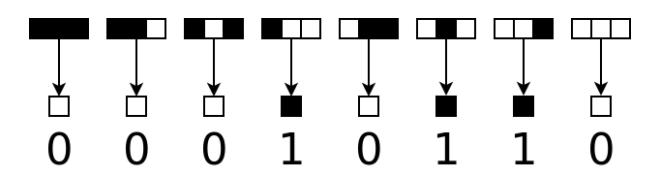
\includegraphics[width=10cm]{imgs/rule_22.png}}
  \caption{Ilustração das regras de transição para a regra 22 no código Wolfram. }
\end{figure}

\tab Os ACEs são enumerados por suas regras de transição, de 0 a 255, o que é conhecido como número de Wolfram. Segundo \cite[p. 24]{wolfram2002new}, ``A linha superior em cada caixa dá uma das possíveis combinações de cores para uma célula e sua vizinhança imediata. A linha inferior então especifica qual será a cor da célula central no próximo passo em cada um desses casos.''

\tab Uma definição direta de regra de transição consiste na enumeração de todas as combinações de estado possíveis da vizinhança de uma célula, e do próximo estado associado a elas, o que define a função local a ser usada na evolução temporal do reticulado.

% \break

\subsection{Atualização Assíncrona por Prioridade da Vizinhança} \label{udsn}
Parte imprescindível da definição de um AC é a ordem de atualização das células no reticulado. Apesar de os ACs serem fundamentalmente concebidos com o comportamento de atualização síncrona, é possível se utilizar das mais diversas e criativas estratégias de atualização.

\tab No presente trabalho foi empregada uma nova estratégia de atualização: por "prioridade da vizinhança", em que os esquemas associados contém a prioridade da atualização de cada uma das 8 possíveis vizinhanças do espaço elementar, as quais deverão ser seguidas deterministicamente durante as evoluções temporais.  

\tab Esse tipo de atualização requer uma distinção das iterações globais e locais (microiterações):  as prioridades de vizinhanças são iteradas sequencialmente de menor a maior e para cada prioridade, o reticulado é varrido e atualizam-se apenas as células que tenham vizinhança com a prioridade atual, mantendo-se o estado das vizinhanças que não estejam na prioridade atual da iteração. Ao fim da varredura do reticulado, o processo se repete para a próxima prioridade, agora iterando sobre o reticulado gerado no processo descrito anteriormente, com uma prioridade menor. O reticulado resultante após iterar sobre todas as prioridades é chamado de iteração global (ou macroiteração) e é incluído nas renderizações, o que não acontece com as microiterações.

\tab Esse modo de atualização inclui também a atualização síncrona, que pode ser simulada quando as prioridades do esquema têm mesmo valor (11111111, 22222222, ..., etc). As evoluções podem ser identificadas como um par $\langle\,R,E\,\rangle$, onde \textit{R} é a regra e \textit{E} é um esquema de prioridade. 

\tab É importante notar que diferentes esquemas de prioridade podem ser equivalentes: quando esquemas de prioridade equivalentes são aplicados a uma mesma regra, são geradas evoluções iguais. Um exemplo entre esquemas equivalentes pode ser entre os esquemas 11111112 e 11111113, em que as prioridades da última transição são nominalmente diferentes, mas efetivamente iguais. Outro caso é a equivalência entre os oito esquemas síncronos: 11111111, 22222222, 33333333, etc. Para experimentos feitos neste trabalho, foram filtrados esses dois casos, de modo que não houvesse redundância nas execuções, reduzindo o custo computacional.

\tab Além desses dois tipos de equivalência entre esquemas, é possível haver equivalência entre esquemas apenas quando são pareados a uma determinada regra, em função de suas transições não-ativas, como é o caso do que acontece no primeiro experimento, discutido na seção \ref{resultados}.

% \break

\subsection{Conservabilidade Numérica} \label{num-conserv}
Segundo \cite{boccara2002number}, ``Uma regra de AC \textit{f} de \textit{q} estados, unidimensional, de comprimento \textit{n} é conservativa se, para todas as configurações cíclicas de tamanho \textit{L} \(\geq\) \textit{n} satisfaz'':

\[f(x_1,x_2,...,x_{n-1},x_n) + f(x_2,x_3,...,x_n,x_{n+1}) + ... \]
\[ + \;   f(x_L,x_1,...,x_{n-2},x_{n-1} = x_1 + x_2 + ... + x_L\] 

\tab No contexto de ACEs, uma evolução é dita conservativa caso, para qualquer configuração inicial, a soma dos estados presentes numa configuração é sempre a mesma para todas as iterações. Como é mencionado na subseção \ref{contex}, ACs conservativos podem ser usados para modelar ambientes em que há conservabilidade, como trânsito automobilístico, simulação de partículas, entre outros. A regra 184 é uma regra que, em execução síncrona, gera evoluções conservativas pela definição anterior de conservabilidade. 
% Na seção \ref{resultados} são apresentados os esquemas em que a regra 184 permanece conservativa com a estratégia de atualização discutida em \ref{udsn}.

\subsection{Classificação de Densidade} \label{dct}
Segundo \cite[p. 1]{capcarrere1996two}, ``um exemplo dessa computação emergente é utilizar um AC para determinar a densidade global de bits em uma configuração de estado inicial. Conhecido como o problema de classificação de densidade, o AC unidimensional de dois estados é apresentado com uma configuração inicial arbitrária e deve convergir no tempo para um estado de apenas 1s se a configuração inicial contiver uma densidade de 1s > 0,5, e de apenas 0s se essa densidade < 0,5; para uma densidade inicial de 0,5, o comportamento do AC é indefinido''. Em outras palavras, capacidade de classificação de densidade se dá quando o reticulado cíclico de um ACE torna-se totalmente preenchido pelo estado predominante na configuração inicial.

\subsection{Problema da Paridade} \label{parity-problem}
Segundo \cite[p. 1]{betel2012parity}, ``Consideramos o problema de paridade em autômatos celulares unidimensionais, binários e circulares: se a configuração inicial contém um número ímpar de 1s, a reticulado inteira deve convergir para 1s; caso contrário, deve convergir para 0s''. Assim como o problema da maioria, ``é fácil ver que o problema é mal-definido para reticulados de tamanho ímpar (que, por definição, nunca seriam capazes de convergir para 1)''. É possível entender, então, que a solução do problema da paridade se dá quando o reticulado cíclico de um ACE torna-se totalmente preenchido pelo estado de quantidade ímpar na configuração inicial.  

\section{Metodologia da Pesquisa}

No que tange à Metodologia empregada neste TCC, o trabalho teve início com uma revisão da literatura específica sobre o tema da pesquisa. Esta pesquisa abrange conceitos fundamentais de teoria da computação e o ``estado da arte'' em termos de análise de conservabilidade.

\tab Este alicerce teórico foi obtido através de autores como: Wolfram; Boccara;
entre outros, além de pesquisas em periódicos científicos, sites, publicações em empresas, teses e dissertações em universidades e publicações de associações técnicas.  A leitura, análise e comparação da fundamentação teórica tiveram início com ACEs síncronos, modificados em seguida para viabilizar o tipo de atualização mencionado na subseção \ref{udsn}.

\tab A capacidade de classificação de densidade e a capacidade de resolução do problema da paridade foram medidas através da contagem de configurações iniciais em que cada par $\langle\,R,E\,\rangle$ resolve o problema em questão.

\subsection{Organização e Delimitação do Estudo} \label{delimitacao}

A pesquisa se limita a ACEs com o tipo de atualização evidenciado na subseção \ref{ref_ace}, com comprimento de reticulados testados até \textit{n}=15 e com \textit{r}=1. 

\tab Para o primeiro experimento, foram testados esquemas de atualização \textit{independentes} para o ACE 184, i.e., os esquemas cujas dinâmicas são definidas pelas transições \textit{ativas} de estado da regra, as que mudam o estado da célula central. 

\tab Os três experimentos foram de natureza computacional. Foram testados comprimentos de reticulado (\textit{n}) sucessivamente maiores, de \textit{n}=5 em diante. Para o primeiro experimento, foram testados esquemas de atualização \textit{independentes} para o ACE 184, i.e., os esquemas cujas dinâmicas são definidas pelas transições \textit{ativas} de estado da regra, as que mudam o estado da célula central. Para o segundo e o terceiro experimento, foram escolhidas regras \textit{balanceadas} (as que têm quatro transições de estado para cada um dos estados, 0 e 1) e que tivessem no máximo 75 esquemas independentes por regra; o balanceamento se deve a uma condição necessária do problema e a restrição em 75 esquemas para diminuir as demandas computacionais.

\break
\section{Resultados dos Experimentos} \label{resultados}

\textbf{Experimento 1}

\tab É sabido que há cinco regras que apresentam conservabilidade numérica em suas evoluções: 170, 184, 204, 226 e 240. A motivação para o primeiro experimento foi descobrir se, no esquema de atualização usado, essa propriedade é mantida para a regra 184 (que é equivalente à regra 226), que foi escolhida por ser a mais rica do ponto de vista dinâmico dentre as cinco, empatada com a 226.

\tab Em relação à conservabilidade, a execução da regra 184 com todas as configurações iniciais de comprimento até \textit{n}=15, e com todos os seus esquemas de prioridade independentes, resultou num conjunto de esquemas assíncronos em que a regra permanece conservativa, como é mostrado na figura \ref{fig:evolucoes}. Nota-se, entretanto, que todos correspondem ao modo síncrono, já que eles só diferem entre si nas prioridades das transições inativas, e as prioridades das ativas são as mesmas em cada esquema.

\begin{figure}[h]
  \begin{minipage}[htb]{.5\linewidth}
    \centering
    \fbox{
\includegraphics[width=0.1\linewidth]{imgs/184-5x33-11111111.png}}
    \caption{Todos os esquemas assíncronos conservativos da regra 184 são equivalentes.}
    \label{fig:evolucoes}
  \end{minipage}%
  \begin{minipage}[htb]{.6\linewidth}
    \centering
    \begin{tabular}{ | c | c | } \hline
      Regra & Esquema  \\\hline 
      \multirow{13}{*}{184} 
	    & \underline{3}222\underline{2}2\underline{21} \\
	    & \underline{3}111\underline{1}1\underline{12} \\      
	    & \underline{2}333\underline{3}3\underline{31} \\      
	    & \underline{2}111\underline{1}1\underline{13} \\      
	    & \underline{1}333\underline{3}3\underline{32} \\      
	    & \underline{1}222\underline{2}2\underline{23} \\      
	    & \underline{2}222\underline{2}2\underline{21} \\      
	    & \underline{2}111\underline{1}1\underline{12} \\      
	    & \underline{2}111\underline{1}1\underline{11} \\      
	    & \underline{1}222\underline{2}2\underline{22} \\      
	    & \underline{1}222\underline{2}2\underline{21} \\      
	    & \underline{1}111\underline{1}1\underline{12} \\      
	    & \underline{1}111\underline{1}1\underline{11} \\       
      \hline
    \end{tabular}
\end{minipage}
\label{fig:test}
\end{figure}

\tab As prioridades com underscore significam que qualquer prioridade pode ser colocada em seu lugar. Isto se deve a, nesses índices, as transições de estado serem não-ativas e, portanto, serem irrelevantes em que ordem são atualizadas.
No entanto, é possível ver que as prioridades das transições de estado ativas são iguais entre si, que são todas representações equivalentes da execução síncrona.

\textbf{Experimentos 2 e 3}

A motivação para os dois últimos experimentos a respeito do problema da maioria e problema da paridade foi estudar se os ACEs com atualização assíncrona por prioridade eram capazes de resolver esses problemas de decisão emblemáticos no contexto de ACs.

\tab A execução das regras e esquemas de prioridade independentes selecionadas até comprimento \textit{n}=7 bastou para mostrar que nenhuma das regras elementares testadas foi capaz de classificar a densidade nem resolver o problema da paridade totalmente, qualquer que fosse o esquema de atualização independente utilizado.

\tab A seguir são apresentadas as regras a quantidade de esquemas testados para elas no presente trabalho.

\break

\begin{center}
% \caption{Primeiro conjunto de regras e quantidade de esquemas testados}
\begin{longtable}{ | c | c | } 
\caption{Primeiro conjunto de regras e quantidade de esquemas testados}\\
  \hline
 Regra & Qtd. Esquemas     \\\hline
  29 & 75  \\ \hline
  30 & 75  \\ \hline
  45 & 75  \\ \hline
  46 & 75  \\ \hline
  60 & 75  \\ \hline
  71 & 75  \\ \hline
  75 & 75  \\ \hline
  77 & 3   \\ \hline
  78 & 3   \\ \hline
  85 & 75  \\ \hline
  86 & 75  \\ \hline
  89 & 75  \\ \hline
  90 & 75  \\ \hline
  92 & 3   \\ \hline
  101 & 75 \\ \hline
  102 & 75 \\ \hline
  105 & 75 \\ \hline
  106 & 75 \\ \hline
  108 & 3  \\ \hline
  116 & 75 \\ \hline
  120 & 75 \\ \hline
  135 & 75 \\ \hline
  139 & 75 \\ \hline
  141 & 3  \\ \hline
  142 & 3  \\ \hline
  149 & 75 \\ \hline
  150 & 75 \\ \hline
  153 & 75 \\ \hline
  154 & 75 \\ \hline
  156 & 3  \\ \hline
  165 & 75 \\ \hline
  166 & 75 \\ \hline
  169 & 75 \\ \hline
  170 & 75 \\ \hline
  172 & 3  \\ \hline
  180 & 75 \\ \hline
  184 & 75 \\ \hline
  195 & 75 \\ \hline
  197 & 3  \\ \hline
  198 & 3  \\ \hline
  201 & 3  \\ \hline
  ... & ... \\ \hline
  ... & ... \\ \hline
  202 & 3  \\ \hline
  204 & 1  \\ \hline
  209 & 75 \\ \hline
  210 & 75 \\ \hline
  212 & 3  \\ \hline
  216 & 3  \\ \hline
  225 & 75 \\ \hline
  226 & 75 \\ \hline
  228 & 3  \\ \hline
  232 & 3  \\ \hline
\end{longtable}
\end{center}
% \break


\begin{center}
  \begin{longtable}{ | c | c | } 
  \caption{Segundo conjunto de regras e quantidade de esquemas testados}\\
    \hline
    Regra & Qtd. Esquemas     	\\\hline
    23 & 4683 \\\hline
    27 & 4683 \\\hline
    % ... & ... \\ \hline
    % ... & ... \\ \hline
    39 & 4683 \\\hline
    43 & 4683 \\\hline
    53 & 4683 \\\hline
    54 & 4683 \\\hline
    57 & 4683 \\\hline
    58 & 4683 \\\hline
    83 & 4683 \\\hline
    99 & 4683 \\\hline
    113 & 4683 \\\hline
    114 & 4683 \\\hline
    147 & 4683 \\\hline
    163 & 4683 \\\hline
    177 & 4683 \\\hline
    178 & 4683 \\\hline
  \end{longtable}
\end{center}

\section{Considerações Finais} \label{comentarios-finais}

Esta pesquisa é um passo no estudo sobre ACEs com atualização assíncrona por prioridade da vizinhança. Para tanto, realizamos os três experimentos acima descritos.

\tab O primeiro experimento mostrou que a regra 184 permanece conservativa apenas em esquemas de atualização equivalentes ao modo síncrono. Já o segundo experimento revelou que, para os esquemas de atualização testados, não havia pares $\langle\,R,E\,\rangle$ que resolvessem o problema da maioria. Por fim, o terceiro experimento demonstrou que não havia pares $\langle\,R,E\,\rangle$ que resolvessem o problema da paridade.

\tab É importante apontar que as conclusões mostradas aqui não incluíram todos os esquemas de atualização possíveis pelo alto custo computacional e que é necessário notar que esta estratégia de atualização é recente e ainda há muitos testes a serem feitos, seja para identificar propriedades estáticas ou verificar a capacidade de resolver problemas de decisão.

\tab A única regra que não foi analisada no contexto dos problemas de decisão discutidos foi a regra 51 (chamada regra inversora, que muda 0s para 1s e vice-versa), e que contém a máxima quantidade possível de esquemas de atualização independentes (545.835 esquemas).

\tab Estudamos três importantes propriedades nos ACEs executados com a estratégia de atualização assíncrona por prioridade da vizinhança: conservabilidade numérica, capacidade de classificação de densidade e capacidade de resolver o problema da maioria. 

% \break

% Queremos agradecer nosso orientador, Prof. Dr. Pedro Paulo Balbi de Oliveira pelo forte, contínuo e atencioso apoio ao longo do desenvolvimento desta pesquisa.

% \addcontentsline{toc}{section}{Referências}
% \bibliography{cellz} \label{bib}
\bibliographystyle{sbc}
\bibliography{cellz}

\end{document}
